\ifdefined\included
\else
\documentclass[english,a4paper,11pt,twoside]{StyleThese}
\usepackage{amsmath,amssymb}             % AMS Math
\usepackage[T1]{fontenc}
\usepackage[utf8x]{inputenc}
\usepackage{babel}
\usepackage{datetime}

\usepackage{lmodern}
\usepackage{tabularx}
%\usepackage{tabular}
\usepackage{multirow}

\usepackage{subfigure}
\usepackage{fancyvrb}
\usepackage{algorithmic}
\usepackage{algorithm}
\usepackage{mathtools}


\usepackage{hhline}
\usepackage[left=1.5in,right=1.3in,top=1.1in,bottom=1.1in,includefoot,includehead,headheight=13.6pt]{geometry}
\renewcommand{\baselinestretch}{1.05}

% Table of contents for each chapter

\usepackage[nottoc, notlof, notlot]{tocbibind}
\usepackage{minitoc}
\setcounter{minitocdepth}{2}
\mtcindent=15pt
% Use \minitoc where to put a table of contents

\usepackage{aecompl}


% Glossary / list of abbreviations

\usepackage[intoc]{nomencl}
\iftoggle{ThesisInEnglish}{%
\renewcommand{\nomname}{Glossary}
}{ %
\renewcommand{\nomname}{Liste des Abréviations}
}

\newcommand{\accom}[1]{\textcolor{red}{[#1]}}

\makenomenclature

% My pdf code

\usepackage{ifpdf}

\ifpdf
  \usepackage[pdftex]{graphicx}
  \DeclareGraphicsExtensions{.jpg}
  \usepackage[a4paper,pagebackref,hyperindex=true]{hyperref}
  \usepackage{tikz}
  \usetikzlibrary{arrows,shapes,calc}
\else
  \usepackage{graphicx}
  \DeclareGraphicsExtensions{.ps,.eps}
  \usepackage[a4paper,dvipdfm,pagebackref,hyperindex=true]{hyperref}
\fi

\graphicspath{{.}{images/}}

%% nicer backref links. NOTE: The flag ThesisInEnglish is used to define the
% language in the back references. Read more about it in These.tex

\iftoggle{ThesisInEnglish}{%
\renewcommand*{\backref}[1]{}
\renewcommand*{\backrefalt}[4]{%
\ifcase #1 %
(Not cited.)%
\or
(Cited in page~#2.)%
\else
(Cited in pages~#2.)%
\fi}
\renewcommand*{\backrefsep}{, }
\renewcommand*{\backreftwosep}{ and~}
\renewcommand*{\backreflastsep}{ and~}
}{%
\renewcommand*{\backref}[1]{}
\renewcommand*{\backrefalt}[4]{%
\ifcase #1 %
(Non cité.)%
\or
(Cité en page~#2.)%
\else
(Cité en pages~#2.)%
\fi}
\renewcommand*{\backrefsep}{, }
\renewcommand*{\backreftwosep}{ et~}
\renewcommand*{\backreflastsep}{ et~}
}

% Links in pdf
\usepackage{color}
\definecolor{linkcol}{rgb}{0,0,0.4} 
\definecolor{citecol}{rgb}{0.5,0,0} 
\definecolor{linkcol}{rgb}{0,0,0} 
\definecolor{citecol}{rgb}{0,0,0}
% Change this to change the informations included in the pdf file

\hypersetup
{
bookmarksopen=true,
pdftitle="Joint Action for Human-Robot Interaction",
pdfauthor="Sandra DEVIN", %auteur du document
pdfsubject="Thesis", %sujet du document
%pdftoolbar=false, %barre d'outils non visible
pdfmenubar=true, %barre de menu visible
pdfhighlight=/O, %effet d'un clic sur un lien hypertexte
colorlinks=true, %couleurs sur les liens hypertextes
pdfpagemode=None, %aucun mode de page
pdfpagelayout=SinglePage, %ouverture en simple page
pdffitwindow=true, %pages ouvertes entierement dans toute la fenetre
linkcolor=linkcol, %couleur des liens hypertextes internes
citecolor=citecol, %couleur des liens pour les citations
urlcolor=linkcol %couleur des liens pour les url
}

% definitions.
% -------------------

\setcounter{secnumdepth}{3}
\setcounter{tocdepth}{2}

% Some useful commands and shortcut for maths:  partial derivative and stuff

\newcommand{\pd}[2]{\frac{\partial #1}{\partial #2}}
\def\abs{\operatorname{abs}}
\def\argmax{\operatornamewithlimits{arg\,max}}
\def\argmin{\operatornamewithlimits{arg\,min}}
\def\diag{\operatorname{Diag}}
\newcommand{\eqRef}[1]{(\ref{#1})}

\usepackage{rotating}                    % Sideways of figures & tables
%\usepackage{bibunits}
%\usepackage[sectionbib]{chapterbib}          % Cross-reference package (Natural BiB)
%\usepackage{natbib}                  % Put References at the end of each chapter
                                         % Do not put 'sectionbib' option here.
                                         % Sectionbib option in 'natbib' will do.
\usepackage{fancyhdr}                    % Fancy Header and Footer

% \usepackage{txfonts}                     % Public Times New Roman text & math font
  
%%% Fancy Header %%%%%%%%%%%%%%%%%%%%%%%%%%%%%%%%%%%%%%%%%%%%%%%%%%%%%%%%%%%%%%%%%%
% Fancy Header Style Options

\pagestyle{fancy}                       % Sets fancy header and footer
\fancyfoot{}                            % Delete current footer settings

%\renewcommand{\chaptermark}[1]{         % Lower Case Chapter marker style
%  \markboth{\chaptername\ \thechapter.\ #1}}{}} %

%\renewcommand{\sectionmark}[1]{         % Lower case Section marker style
%  \markright{\thesection.\ #1}}         %

\fancyhead[LE,RO]{\bfseries\thepage}    % Page number (boldface) in left on even
% pages and right on odd pages
\fancyhead[RE]{\bfseries\nouppercase{\leftmark}}      % Chapter in the right on even pages
\fancyhead[LO]{\bfseries\nouppercase{\rightmark}}     % Section in the left on odd pages

\let\headruleORIG\headrule
\renewcommand{\headrule}{\color{black} \headruleORIG}
\renewcommand{\headrulewidth}{1.0pt}
\usepackage{colortbl}
\arrayrulecolor{black}

\fancypagestyle{plain}{
  \fancyhead{}
  \fancyfoot{}
  \renewcommand{\headrulewidth}{0pt}
}

%\usepackage{MyAlgorithm}
%\usepackage[noend]{MyAlgorithmic}
\usepackage[ED=MITT - STICIA, Ets=INP]{tlsflyleaf}
%%% Clear Header %%%%%%%%%%%%%%%%%%%%%%%%%%%%%%%%%%%%%%%%%%%%%%%%%%%%%%%%%%%%%%%%%%
% Clear Header Style on the Last Empty Odd pages
\makeatletter

\def\cleardoublepage{\clearpage\if@twoside \ifodd\c@page\else%
  \hbox{}%
  \thispagestyle{empty}%              % Empty header styles
  \newpage%
  \if@twocolumn\hbox{}\newpage\fi\fi\fi}

\makeatother
 
%%%%%%%%%%%%%%%%%%%%%%%%%%%%%%%%%%%%%%%%%%%%%%%%%%%%%%%%%%%%%%%%%%%%%%%%%%%%%%% 
% Prints your review date and 'Draft Version' (From Josullvn, CS, CMU)
\newcommand{\reviewtimetoday}[2]{\special{!userdict begin
    /bop-hook{gsave 20 710 translate 45 rotate 0.8 setgray
      /Times-Roman findfont 12 scalefont setfont 0 0   moveto (#1) show
      0 -12 moveto (#2) show grestore}def end}}
% You can turn on or off this option.
% \reviewtimetoday{\today}{Draft Version}
%%%%%%%%%%%%%%%%%%%%%%%%%%%%%%%%%%%%%%%%%%%%%%%%%%%%%%%%%%%%%%%%%%%%%%%%%%%%%%% 

\newenvironment{maxime}[1]
{
\vspace*{0cm}
\hfill
\begin{minipage}{0.5\textwidth}%
%\rule[0.5ex]{\textwidth}{0.1mm}\\%
\hrulefill $\:$ {\bf #1}\\
%\vspace*{-0.25cm}
\it 
}%
{%

\hrulefill
\vspace*{0.5cm}%
\end{minipage}
}

\let\minitocORIG\minitoc
\renewcommand{\minitoc}{\minitocORIG \vspace{1.5em}}

\usepackage{multirow}
%\usepackage{slashbox}

\newenvironment{bulletList}%
{ \begin{list}%
	{$\bullet$}%
	{\setlength{\labelwidth}{25pt}%
	 \setlength{\leftmargin}{30pt}%
	 \setlength{\itemsep}{\parsep}}}%
{ \end{list} }

\newtheorem{definition}{Définition}
\renewcommand{\epsilon}{\varepsilon}

% centered page environment

\newenvironment{vcenterpage}
{\newpage\vspace*{\fill}\thispagestyle{empty}\renewcommand{\headrulewidth}{0pt}}
{\vspace*{\fill}}

\usepackage{tablefootnote}

\sloppy
\begin{document}
\dominitoc
\faketableofcontents
\fi


\chapter*{Introduction}
\addstarredchapter{Introduction} %Sinon cela n'apparait pas dans la table des matières
\minitoc

\section*{Context}
\addcontentsline{toc}{section}{Context}

In the 1940s, researchers invented the first machines that we can call computers. Then, they quickly came to think that, this new tool which can easily manipulate numbers can also manipulate symbols, and they started to work on new "thinking machines". In 1956, at the Dartmouth conference, the domain of "Artificial Intelligence" is recognized as a fully academic field. Associated to the automaton technology, the first "robots" quickly arrived in our environment.

Some of these robots are meant to work alone (e.g. rovers for space exploration) while others need to work in the vicinity and/or with humans. One possible example is robot "co-workers". These robots need to collaborate in a safe, efficient and fluent way with humans to accomplish more or less repetitive tasks. The last decades also witnessed the apparition of what is called "sociable robots" \cite{dautenhahn2007socially}. These robots can be used, for example, to help elderly or injured people in their daily life our to guide people in public spaces. 

The aim of this thesis is to make a step toward robots which act jointly with humans in a natural, efficient and fluent way. We focus more especially on the decisional issues that can appear during a human-robot Joint Action. The subject of Joint Action between humans has been studied a lot in social sciences, however, many things remain to be discovered. Based on these results, the aim here is to build robots which are able to understand the humans (their beliefs and choices) and to adapt to them in order to be more pleasant and efficient companions.

\section*{Contributions and manuscript organization}
\addcontentsline{toc}{section}{Contributions and manuscript organization}

In order to endow the robot with decisional abilities during Joint Action with humans, we bring several contributions to the field which are presented in the manuscript as follow:
\begin{itemize}
\item In a first part, we study the basis of the Joint Action principles in order to build a supervisor for human-robot Joint Action. 
\begin{itemize}
\item In Chapter~\ref{ch:biblio}, we first study the bibliography about Joint Action between humans in social science in order to identify what are the needed components for a robot decision adapted to Joint Action. Secondly, we look how these components have already been applied in robotics and, finally, we study how to articulate all these components and how, inspired by models from philosophy, we can build a robotics architecture for human-robot interaction.
\item In Chapter~\ref{ch:Sup}, we present the supervisor for human-robot collaboration which has been developed during the thesis. This supervisor is the main technical contribution of the thesis.
\end{itemize}
\item In a second part, we focus on the achievement by a robot of a \textit{Shared Plan} in collaboration with a human:
\begin{itemize}
\item In Chapter~\ref{ch:MS}, we present how we endowed the robot with the ability to estimate the humans mental states, not only about the environment, but also concerning the state of the task and more particularly of the Shared Plan. We also show how we use these mental states to allow the robot to better communicate about divergent beliefs during Shared Plan execution.
\item In Chapter~\ref{ch:SP}, we describe the work done in order to allow the robot to gain acceptability and fluency during Shared Plan achievement by working with more flexible Shared Plans. We first identified the needed decisions during Shared Plan elaboration and execution and we endow the robot with the ability to decide which decisions should be taken at planning time and which one are better postponed at execution time. Then, we allowed the robot to take these decision by smoothly adapting to the human choices.
\item Finally, in Chapter~\ref{ch:Eval}, we evaluate the new implemented system for the achievement of human-robot Shared Plan. This evaluation has been done quantitatively in simulation but also qualitatively with a user study with the real robot.
\end{itemize} 
In the last part, we present other contributions to the subject:
\begin{itemize}
\item In Chapter~\ref{ch:Acting}, we study the non-verbal behavior, and more especially the head -gaze- behavior, needed during Joint Action between humans and between a human and a robot. We identify the needed components of a robot head behavior adapted to the Joint Action and studied more deeply some of them with an on-line video based study. Finally, we present how these components can be implemented into a robot head behavior architecture.
\item In Chapter~\ref{ch:Learning}, inspired from studies in neuroscience, we combine learning and planning for high level decisions during human-robot Joint Action. The idea it to take advantage from both sides in order to come up with decision level which is able to quickly learn how to smoothly adapt to the human choices during Joint Action execution.
\end{itemize}
\end{itemize}

\section*{Work environment}
\addcontentsline{toc}{section}{Work environment}

This thesis has been realized at LAAS-CNRS in the RIS team (Robotics and InteractionS). It was included in the general objective to build a robotics architecture for an autonomous robots which interacts with humans. 

\paragraph{Robot:} in all this thesis, for practical reasons, the developed algorithms have been implemented in a PR2 robot from Clearpath Robotics (previously Willow Garage)\footnote{http://wiki.ros.org/Robots/PR2}. However, these algorithms are generic enough to be implemented in other robots. The PR2 robot is a semi-humanoid robot which is able to navigate and manipulate objects (see Fig.\ref{fig:PR2}).

\begin{figure}[!h]
	\centering
    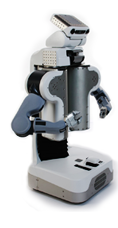
\includegraphics[width=0.3\textwidth]{figs/Introduction/PR2.png}
    \caption{The PR2 robot.}
    \label{fig:PR2}
\end{figure}

\paragraph{Humans and objects detection:} When interacting with humans during manipulation tasks, the robot needs to be able to localize and identify humans and objects. To avoid as much as possible perceptions issues which are not the focus of this thesis, the perception of humans and objects is simplified here. The humans are identified and perceived thanks to a motion capture system. They wear a helmet to get the position and orientation of their heads and a glove to get the position and orientation of their right hands (see Fig.~\ref{fig:Environment}). Concerning the objects, they are identified and localized with tags thanks to the robot cameras in its head.

\begin{figure}[!h]
	\centering
    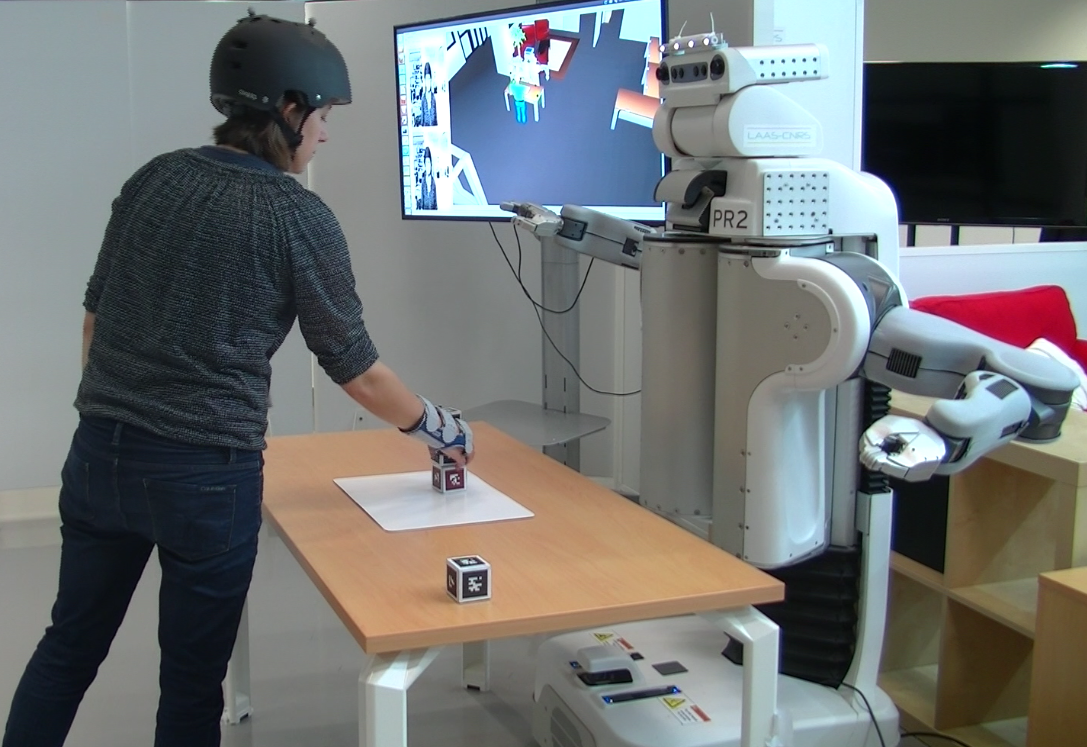
\includegraphics[width=0.7\textwidth]{figs/Introduction/SetUp.png}
    \caption{The PR2 robot interacting with a human to build a stack of cubes. The human is detected thanks to a motion capture system (helmet and glove) and the objects with tags.}
    \label{fig:Environment}
\end{figure}

\section*{Publications}
\addcontentsline{toc}{section}{Publications}

The work presented in this thesis has led to several publications. They are listed here bellow (from the most recent to the oldest):
\begin{itemize}
\item \textbf{Devin, S.}, Clodic, A., Alami, R. (2017). About Decisions During Human-Robot Shared Plan Achievement: Who Should Act and How? The Ninth International Conference on Social Robotics. \textit{Submitted}.
\item \textbf{Devin, S.}, Alami, R. (2016). An implemented theory of mind to improve human-robot shared plans execution. In Human-Robot Interaction (HRI), 2016 11th ACM\/IEEE International Conference on (pp. 319-326). IEEE.
\item \textbf{Devin, S}., Milliez, G., Fiore, M., Clodic, A., Alami, R. (2016). Some essential skills and their combination in an architecture for a cognitive and interactive robot. Workshop In Human-Robot Interaction (HRI), 2016 11th ACM\/IEEE International Conference on (pp. 319-326). IEEE.
\item Khamassi, M., Girard, B., Clodic, A., \textbf{Sandra, D.}, Renaudo, E., Pacherie, E., Alami, R., Chatila, R. (2016). Integration of Action, Joint Action and Learning in Robot Cognitive Architectures. Intellectica (ARCo), 2016(65), 169-203.
\item Renaudo, E., \textbf{Devin, S.}, Girard, B., Chatila, R., Alami, R., Khamassi, M., Clodic, A. (2015). Learning to interact with humans using goal-directed and habitual behaviors. In RoMan 2015, Workshop on Learning for Human-Robot Collaboration.
\end{itemize}


\ifdefined\included
\else
\bibliographystyle{StyleThese}
\bibliography{These}
\end{document}
\fi